\chapter{Informationsteoretiske Nedre Grænser og Modstander Nedre Grænser for sortering ved sammenligninger}

\section{Informationsteoretisk Nedre Grænse}%
\label{sec:label}

\begin{note}[Kilder]
  Video 24\\
  \href{https://imada.sdu.dk/u/jbj/DM553/Baaselowerbound.pdf}{Baase}
\end{note}

Vi vil i dette delkapitel bevise en nedre grænse på $n \log n$ for sammenligningsbaseret sorteringsalgoritmer, ved hjælp af \textit{decision træer}. Hver deterministisk sammenligningsbaseret sorteringsalgoritme $A$ kan blive associeret med et decision træ. Et decision træ, er et træ hvor knuderne er sammenligninger, og kanterne repræsenterer resultatet af en sammenligning.


\begin{figure}[ht]
  \centering
\begin{tikzpicture}[node distance=3cm and 6cm]

\tikzstyle{decision} = [ellipse, draw, text centered, minimum height=1cm]
\tikzstyle{arrow} = [thick,->,>=stealth]

% Nodes
\node (root) [decision] {$X_{13} < X_{17}$};
\node (left1) [decision, below left of=root, xshift=-2cm] {$X_{7} < X_{12}$};
\node (right1) [decision, below right of=root, xshift=2cm] {$X_{8} < X_{9}$};

% Leaves for left1
\node (left1left) [below left of=left1, xshift=-1cm] {};
\node (left1right) [below right of=left1, xshift=1cm] {};

% Leaves for right1
\node (right1left) [below left of=right1, xshift=-1cm] {};
\node (right1right) [below right of=right1, xshift=1cm] {};

% Paths
\draw [arrow] (root) -- node[anchor=east] {N} (left1);
\draw [arrow] (root) -- node[anchor=west] {Y} (right1);
\draw [arrow] (left1) -- node[anchor=east] {N} (left1left);
\draw [arrow] (left1) -- node[anchor=west] {Y} (left1right);
\draw [arrow] (right1) -- node[anchor=east] {N} (right1left);
\draw [arrow] (right1) -- node[anchor=west] {Y} (right1right);

% Leaf nodes
\draw (left1left) node[rectangle, draw] {};
\draw (left1right) node[rectangle, draw] {};
\draw (right1left) node[rectangle, draw] {};
\draw (right1right) node[rectangle, draw] {};

\end{tikzpicture}
  \caption{\label{fig:decisiontree} Eksempel på et decision træ.}
\end{figure}

I Figur~\ref{fig:decisiontree} ses et eksempel på et decision træ, som har tre knuder. Den første spørger om element $X_{13}$ er mindre end $X_{17}$. Hvis svaret er ja, går den videre til knuden i højre siden, og ellers knuden i venstre. Dette mønster, hvor hvis svaret er ``ja'' går den til højre, og ellers venstre, fortsætter igennem træet. Dette korte træ, som næppe kan repræsentere en hel sortering, har 4 resultater, vist med $\square$ repræsenterer en unik permutation af elementerne der bliver sammenlignet, og er et blad i træet.

Da hver permutation af tallene elementerne $\{1, 2, \ldots, n\}$ skal være et muligt blad, betyder det at der \textbf{mindst} er $n!$ blade. Det er dog muligt at der er flere blade med samme indhold. Vi kalder decision træet for en algoritme $A$ for $T_{A}$. Da $T_{A}$ er et binært træ, betyder det at der er højest $2^{h}$ blade, hvis $T_{A}$ har højde $h$. Dermed $2^{h} \ge n!$, hvilket betyder at $h \ge \log_{2}n! \approx n \log n - cn$.

Hver vej, $P$, fra roden af $T_{A}$ til et blad svarer til de sammenligninger lavet af $A$ til at sortere et input, og antallet af sammenligninger er lig med længden af $P$. Så $A$ bruger mere end $n \log n - cn$ sammenligninger på et input. Det vil altså sige, at i \textit{worst case}, skal der bruges \textit{mindst} $n \log_{2} n - cn$ sammenligninger. Note: Baase siger $n \log_{2} n - \frac{3}{2}n$, jeg er ikke klar over hvorfor jørgen lader det være en ukendt værdi $c$.

Lad $P$ være mængden af alle veje $p$ fra roden til et blad i $T_{A}$. Lad $\ell(P)$ være længden af vej $p$.

\begin{definition}
  External Path Length (EPL) er summen af længden af alle veje fra roden til et blad.
  \begin{equation}
	epl = \sum_{p \in P} \mathit{length}(p)
  \end{equation}
\end{definition}

\begin{lemma}
External Path Length er minimeret, når $T$ er \textit{næsten} balanceret. Det vil sige, at forskellen i højde for 2 blade er højest 1. Altså $\forall p,q$ hvor $p$ og $q$ er blade, gælder det at $|h(p) - h(q)| \le 1$, hvor $h(x)$ er niveauet for knude $x$.
\end{lemma}

\begin{figure}[ht]
  \centering
  \begin{tikzpicture}[node distance=1.5cm and 2cm]

\tikzstyle{node} = [circle, draw, text centered, minimum size=0.6cm]
\tikzstyle{arrow} = [thick,-]

% Left tree
\node (root1) [node] {};
\node (left1) [node, below left of=root1] {};
\node (right1) [node, below right of=root1] {X};
\node (left2) [node, below of=left1] {$\vdots$};
\node (left3) [node, below of=left2] {Y};
\node (left4) [node, below left of=left3, xshift=0.5cm] {};
\node (right4) [node, below right of=left3, xshift=-0.5cm] {};

% Paths for left tree
\draw [arrow] (root1) -- (left1);
\draw [arrow] (root1) -- (right1);
\draw [arrow] (left1) -- (left2);
\draw [arrow] (left2) -- (left3);
\draw [arrow] (left3) -- (left4);
\draw [arrow] (left3) -- (right4);

\node at (2.3, -1) {Level $k$};
\node at (-3, -4) {Level $d-1$};
\node at (-3, -5) {Level $d$};

% Right tree
\node (root2) [node, right of=root1, xshift=7cm] {};
\node (left2_1) [node, below left of=root2] {};
\node (right2_1) [node, below right of=root2] {X};
\node (left2_2) [node, below of=left2_1] {$\vdots$};
\node (left2_3) [node, below of=left2_2] {Y};
\node (right2_2) [node, below left of=right2_1, xshift=0.5cm] {};
\node (right2_3) [node, below right of=right2_1, xshift=-0.5cm] {};

% Paths for right tree
\draw [arrow] (root2) -- (left2_1);
\draw [arrow] (root2) -- (right2_1);
\draw [arrow] (left2_1) -- (left2_2);
\draw [arrow] (left2_2) -- (left2_3);
\draw [arrow] (right2_1) -- (right2_2);
\draw [arrow] (right2_1) -- (right2_3);

\node at (6, -1) {Level $k$};
\node at (6, -2) {Level $k+1$};
\node at (5.9, -4) {Level $d-1$};


\end{tikzpicture}
  \caption{\label{fig:decreaseepl} En måde at reducere \textit{epl} på.}
\end{figure}

\begin{proof}
  I Figur~\ref{fig:decreaseepl} kan vi se et eksempel på hvordan man kan gøre et træ mere balanceret. Man tager to blade fra en knude på det laveste nivea, og giver dem til et blad der er på et højere niveau.

  Altså fjerner vi to veje af længde $2d$ fra træet, samt en vej af længde $k$ fra træet. Vi tilføjer til gengæld to veje af længde $k+1$, og en af længde $d-1$. Dermed er den totale \textbf{reducering} $2d+k - (2(k+1)+d) > 0$, da $k \le d - 2$. Altså er reduceringen større end 0. Jørgen beskriver det omvendt. EPL'en \textit{stiger} med $2(k+1)-k + (d-1-2d) = k+1-d < 0$, altså er \textit{stigningen mindre end 0}, i.e. negativ. Dermed må \textit{epl} være minimum når træet {er} \textit{næsten} balanceret.
\end{proof}

\begin{lemma}
Minimums \textit{epl}'en i et binært træ med $\ell$ blade er $\ell \lfloor \log \ell \rfloor + 2 ( \ell - 2^{\lfloor \log \ell \rfloor} )$
\end{lemma}

\begin{proof}
  Hvis $\ell = 2^{k}$, så $2^{k} \cdot \lfloor \log 2^{k} \rfloor + 2(2^{k} - 2^{k}) = 2^{k} \cdot k $, altså $n \log n$. Hvis $\ell \ne 2^{k}$, så er dybden af træet $d = \lceil \log \ell \rceil $ og $d-1 = \lfloor \log_{2} \ell \rfloor$.

  Antallet af blade på niveau $d$, som er det nederste niveau, er $2(\ell - 2^{d-1})$, altså hvor du tager det totale antal blade, og fjerner antallet af blade fra det tidligere niveau, og ganger med 2, da der er 2 børn per knude som ikke er et blad i niveau $d-1$. Dermed er \textit{epl}'en $\ell(d-1) + 2(\ell-2^{d-1}) = \ell \lfloor \log \ell \rfloor + 2(\ell - 2^{\lfloor \log \ell \rfloor})$
\end{proof}

\begin{lemma}
  Den gennemsnitlige længde af en vej i et binært træ med $\ell$ blade er mindst $\lfloor \log \rfloor$
\end{lemma}

\begin{proof}
  Den mindste gennemsnitlige vej er
  \begin{equation*}
\frac{\ell \lfloor \log \ell \rfloor + 2(\ell - 2^{\lfloor \log \ell \rfloor})}{\ell} = \lfloor \log \ell \rfloor + \varepsilon
  \end{equation*}
  $0 \le \varepsilon < 1 $, da $\ell - 2^{\lfloor \log \ell \rfloor} < \ell/2$.
\end{proof}

\begin{theorem}
Det gennemsnitlige antal af sammenligninger lavet af en algoritme til at sortere $n$ tal gennem sammenligninger er mindst $\lfloor \log n! \rfloor = \Omega(n \log n)$
\end{theorem}

\section{Modstander nedre grænse ved permutationer}%
\label{sec:label}

Vi introducerer her en utroligt simpel, men også utroligt kraftig modstander. Modstanderen har mulig for \textit{altid} at vdejligeholde en liste \(\delta\) som indeholder \textbf{alle} permutationer af inputtet, konstistent med hvilke svar der er givet indtil videre (e.g., hvis 2 er blevet vist til at være det laveste tal, så fjerner modstanderen alle lister der starter med 2). Vi lader \(\delta_{i}\) være permutationen der stadig er mulig efter den $i$'e sammenligning. Dermed er $|\delta_{0}| = n!$.

Strategien for modstanderen er, når vedkommende skal svare på spørgsmålet ``$x < y$?'' i skridt $i$, at vedkommende svarer så størrelsen på listen \textit{højest} halveres, altså $\frac{|\delta_{i}|}{|\delta_{i-1}|} \ge \frac{1}{2}$. Da antallet af mulige permutationer er $n!$, og listen højest halveres ved hvert skridt, vil det tage \textit{mindst} $\log_{2}n!$ sammenligninger før inputtet er sorteret, i.e. $|d_{k}| = 1$. Dermed skal $A$ mindst bruge $n \log n - cn$ sorteringer på et input.



\section{En $\Omega (n \log n)$ nedre grænse til sortering ved sammenligninger}%
\label{sec:sorteringsalgoritmesammenligninger}

\begin{note}[Kilder]
	Video 24 \\
	\href{https://imada.sdu.dk/u/jbj/DM553/LBnoteJBJ21.pdf}{Kapitel 7 - Jørgens noter til nedre grænser}
\end{note}

Vores mål her er at vise at en modstander altid vil kunne tvinge $\frac{1}{2}n \log n$ sammenligninger i enhver sammenligningsbaseret sorteringsalgoritme. Vi antager at listen der skal sorteres har størrelse $n$, og at $n = 2^{k}$, for et ikke-negativt heltal $k$.Modstanderen har, til at lave sin strategi, et binært træ $T$ af dybde $k = \log n$, hvis knuder indeholder elementer. Til at starte med er det kun roden i træet, hvis størrelse ikke er 0, den indeholder nemlig de $n$ elementer der skal sorteres.

Vi giver træet ``niveauer'', sålede at niveau 0 indeholder roden, og niveau $\ell$ indeholder $2^{\ell}$ ``poser''.\footnote{Poser er en anden måde at sige knuder på, vi bruger poser til at betyde knuder der kan indeholde elementer.} Et deltræ $T[b]$ er et deltræ hvor roden er knuden $b$. Ethvert deltræ $T[b]$ på niveau $\ell$ har den invariant, at størrelsen $|T[b]| \le 2^{k-\ell} = \frac{n}{2^{\ell}}$.\footnote{Invariant betyder at udsagnet som følger holder igennem hele algoritmen.}

I algoritmen som modstanderen bruger når vedkommende svarer på en sammenligning, bevæger hvert element sig ned igennem træet, indtil alle $n$ elementer er i deres egen private pose, af størrelse $1$ på niveau $k-1$.\footnote{$k-1$ fordi roden er niveau $0$ og dybden er $k$.} Når dette sker, er alle elementerne sorteret.

Vi definerer tre tilstande, som en pose $b$ kan være i igennem køringen af algoritmen:
\begin{itemize}
	\item \textbf{Åben}: Både venstre og højre deltræ af $b$  har mindre end $2^{k-\ell-1}$ elementer.
	\item \textbf{Højre-flushed}: Venstre deltræ har størrelse $2^{k-\ell-1}$.
	\item \textbf{Venstre-flushed}: Højre deltræ har størrelse $2^{k-\ell-1}$.\footnote{Jørgens noter har nogle fejl i, som han ikke forklarer i videoen. Jeg har valgt at sige at ``venstre-flush'', betyder at elementerne kan komme ned til venstre deltræ. Derudover forklarer han slet ikke i noterne hvad hhv. right og left-flush er, han antager bare at man ved det.}
\end{itemize}

I Figur~\ref{fig:flushes} ses de tre tilstande for en pose $b$.

\begin{figure}[ht]
	\centering
	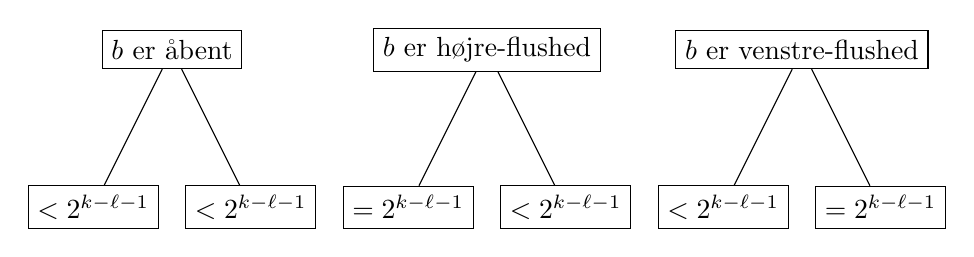
\begin{tikzpicture}[level distance=2cm, sibling distance=2.5cm, every node/.style = {shape=rectangle, draw, align=center}]
		% Open state
		\node at (-4,0) {$b$ er åbent} [sibling distance=2.0cm]
		child {node {$<2^{k-\ell-1}$}}
		child {node {$<2^{k-\ell-1}$}};

		% Left-flushed state
		\node at (0,0) {$b$ er højre-flushed} [sibling distance=2.0cm]
		child {node {$=2^{k-\ell-1}$}}
		child {node {$<2^{k-\ell-1}$}};

		% Right-flushed state
		\node at (4,0) {$b$ er venstre-flushed} [sibling distance=2.0cm]
		child {node {$<2^{k-\ell-1}$}}
		child {node {$=2^{k-\ell-1}$}};
	\end{tikzpicture}
	\caption{\label{fig:flushes} De 3 tilstande $b$ kan være i.}
\end{figure}

Til at udføre sin strategi, gør modstanderen brug af følgende funktioner:
\begin{itemize}
	\item \textbf{MOVE(u)}: Denne funktion kaldes når et element $u$ er kommet til posen $b'$, og gør som følger:
	      \begin{itemize}
		      \item Hvis $b'$ er \textbf{åbent} forbliver $u$ i $b'$.
		      \item Hvis $b'$ er \textbf{højre-flushed} eller \textbf{venstre-flushed} bliver elementet $u$ flyttet til posen $b'$ på hhv. højre eller venstre deltræ. Derefter bliver \textbf{MOVE(u)} kaldt igen.
	      \end{itemize}
	\item \textbf{CHECK(u)}: Denne funktion kaldes ved en åben pose $b$, og gør som følger:
	      \begin{itemize}
		      \item Tjekker om enten højre eller venstre deltræ $T[b]$ af posen $b$ på niveau $\ell$ indeholder $2^{k-\ell-1}$ elementer, og hvis så, markerer den pose $b$ hhv. venstre eller højre-flushed.
		      \item Kalder \textbf{MOVE} på \textit{alle} elementer i $b$.
	      \end{itemize}
\end{itemize}

I Algoritme~\ref{alg:move} og Algoritme~\ref{alg:check} kan algoritmiske fortolkninger ses af hhv. CHECK og MOVE.

\begin{algorithm}
	\caption{\label{alg:move} MOVE(u)}
	\begin{algorithmic}[1]
		\STATE $b(u)$ \COMMENT{Nuværende pose af $u$}
		\IF{$b(u)$ er åben}
		\RETURN
		\ELSIF{$b(u)$ er venstre-flushed}
		\STATE $b(u) \gets b^L(u)$
		\STATE MOVE($u$)
		\RETURN
		\ELSIF{$b(u)$ er højre-flushed}
		\STATE $b(u) \gets b^R(u)$
		\STATE MOVE($u$)
		\RETURN
		\ENDIF
	\end{algorithmic}
\end{algorithm}

\begin{algorithm}
	\caption{\label{alg:check} CHECK(b)}
	\begin{algorithmic}[1]
		\STATE $b$ er en åben pose på niveau $\ell$
		\IF{$|T[b^R]| = 2^{k-\ell-1}$}
		\STATE Marker $b$ som venstre-flushed \COMMENT{højre undertræ er fyldt}
		\STATE MOVE($u$)
		\RETURN
		\ENDIF
		\IF{$|T[b^L]| = 2^{k-\ell-1}$}
		\STATE Marker $b$ som højre-flushed \COMMENT{venstre undertræ er fyldt}
		\STATE MOVE($u$)
		\RETURN
		\ENDIF
		\RETURN
	\end{algorithmic}
\end{algorithm}

\subsection{Modstanderens Strategi}%
\label{subsec:label}

Imens modstanderen svarer på spørgsmål om $x < y$ fra algoritmen, så flytter den enten 2, 1, eller 0 elementer ned i træet, men \textbf{en undtagelse}: Efter hvert \textit{MOVE(u)} kald på et element $u$ fra posen $b$, kalder vi \textit{CHECK(b)}, som kan flytte op til $2^{k-\ell -1}$ elementer. Efter hver query som resulterer i at mindst et element flyttes, kaldes \textit{MOVE(u)} rekursivt på elementet.

Antag at sorteringsalgoritmen $A$ efterspørger resultatet på en sammenligning af elementer $u$ og $v$. Lad \(\ell(u)\) og \(\ell(v)\) være niveauene af hhv. $l$ og $v$. Lad $b(u)$ og $b(v)$ være poserne der indeholder henholdvis $u$ og $v$.

\begin{enumerate}
	\item Hvis den mindste fælles forfader (least comon ancestor) $b$ af $b(u)$ og $b(v)$ i $T$ ikke er $b(u)$ eller $b(v)$, så svarer modstanderen ``$u < v$'' hvis $u$ er i det venstre undertræ af $b$ og $v$ i det højre, og ``$v < u$'', hvis $u$ er i det højre undertræ af $b$ og $u$ i det venstre. Intet element flyttes her. $A$ får ingen information ud af den her sammenligning.
	\item Hvis den mindste fælles forfader $b$ af $b(u)$ og $b(v)$ er i $\{b(u), b(v)\}$, så kan man, uden tab af generalitet, sige at $b = b(u)$ eller $b = b(v)$. Vi antager herfra at $b = b(u)$.
	      \begin{enumerate}
		      \item Hvis $b(u) = b(v)$ så:
		            \begin{itemize}
			            \item Svar ``$u < v$'' og flyt $u$ til roden af det venstre undertræ af $T[b]$, og $v$ til roden af det højre undertræ af $T[b]$.
			            \item Kald \textbf{MOVE(u)}, \textbf{MOVE(v)} og sidst \textbf{CHECK(b)}.
		            \end{itemize}

		      \item Hvis $b(u) \ne b(v)$ og $b(v)$ er i højre undertræ af $b(u)$:
		            \begin{itemize}
			            \item Svar ``$u < v$'' og flyt $u$ til roden at det venstre undertræ af $T[b(u)]$.
			            \item Kald \textbf{MOVE(u)} og så \textbf{CHECK(b)}
		            \end{itemize}
		      \item Hvis $b(u) \ne b(v)$ og $b(v)$ er i venstre undertræ af $T[b(u)]$:
		            \begin{itemize}
			            \item Svar ``$u > v$'', flyt $u$ til roden af det højre deltræ af $T[b(u)]$.
			            \item Kald \textbf{MOVE(u)} og så \textbf{CHECK(b)}
		            \end{itemize}
	      \end{enumerate}
\end{enumerate}

En formulering af algoritmen i \textit{algorithmic} miljøet kan findes i Algoritme~\ref{alg:sortingquery}.

\begin{algorithm}
	\caption{\label{alg:sortingquery} Svar på forespørgsel $u < v$}
	\begin{algorithmic}[1]
		\STATE Lad $b$ være den fælles forfader til $b(u)$ og $b(v)$ i $T$
		\IF{$b \neq b(u)$ og $b \neq b(v)$}
		\IF{$u \in T[b^L]$}
		\STATE svar $u < v$
		\ELSE
		\STATE svar $u > v$
		\ENDIF
		\ELSE
		\STATE \COMMENT{Lad os antage $b = b(v)$, ellers omnavngiv $u,v$}
		\IF{$b(u) = b(v)$}
		\STATE svar $u < v$ og $b(u) \gets b^L(u)$; $b(v) \gets b^R(u)$
		\STATE MOVE($u$); MOVE($v$); CHECK($b$)
		\ELSIF{$b(u)$ i $T[b^R(v)]$}
		\STATE svar $u < v$; $b(u) \gets b^L(u)$
		\STATE MOVE($u$); CHECK($b$)
		\ELSE
		\STATE svar $u > v$; $b(u) \gets $ $b^R(u)$
		\STATE MOVE($u$); CHECK($b$)
		\ENDIF
		\ENDIF
	\end{algorithmic}
\end{algorithm}

\begin{theorem}
	Ved strategien fra Algoritme~\ref{alg:sortingquery}, kan modstanderen tvinge enhver sorteringsbaseret algoritme $A$ til at lave $\Omega(n \log n)$ sammenligninger.
\end{theorem}
\begin{proof}
	Til at starte med har rodposen på niveau $0$ alle $n$ elementer og i slutningen er alle elementer i bladposer på niveau $k = \log n$. \footnote{Tidligere siger Jørgen at dette er $k-1$, han blander nok roden til at være på niveau $0$ og $1$.} I løbet af denne proces får alle andre poser mindst ét element, og bliver så tomme igen, hvilket sker \textit{mindst} én gang.

	Vi viser nu, at vi kan associere mindst $2^{k-\ell-1}$ sammenligninger lavet af algoritmen A privat til hver pose på niveau \(\ell\). Dette betyder, at mindst n/2 sammenligninger associeres privat med hver af de \(\log n\) niveauer, hvilket betyder, at A laver \(\Omega(n \log n)\) sammenligninger før inputtet sorteres. Vi får \(n/2\) fra, at hvert niveau har \(2^{\ell}\) poser, og hver pose bruger mindst \(2^{k-\ell-1}\) sammenligninger, dermed \(2^{\ell} \cdot 2^{k-\ell-1} = 2^{k-1} = n/2\) sammenligninger.

	Lad \( b \) være en arbitrær pose på niveau \( \ell \). Vi viser nu, hvordan man kan associere en mængde af mindst \( 2^{k-\ell-1} \) private sammenligninger af \( A \) til \( b \). Private sammenligninger er sammenligninger, der kun gælder en pose, \( b \). Disse vil være sammenligningerne mellem elementer \( u \) og \( v \), hvor mindst en af elementerne hører til \( b \) og den anden til \( T[b] \) (og dermed muligvis også til \( b \)). Før at \( b \) kan blive flushed (venstre eller højre) og dermed være færdig med sammenligninger i \( b \), skal et af undertræerne have \( 2^{k-\ell-1} \) elementer. Disse elementer skal flyttes ned i træet, hvilket sker via sammenligninger. Dermed kræves der mindst \( 2^{k-\ell-1} \) sammenligninger for en pose \( b \).
\end{proof}

\begin{corollary}
	Modstanderens strategi kan gøres i tid $O(n \log n)$.
\end{corollary}

\begin{proof}
	Repræsentationen af $T$ kan implementeres ved at lade de $2^{\ell}$ poser på niveau $\ell$ repræsenteres som $b_{\ell,0 }, b_{\ell, 1}, \ldots, b_{\ell, 2^{\ell}-1}$, og ved at holde to værdier for hvert element $u$: $\ell(u)$ og $b(u)$, hvor $0 \le b(u) \le 2^{\ell(u)}-1$. Hvis $u$ flyttes ned på et niveau i det venstre (hhv. højre) undertræ af $b(u)$ erstatter vi $b(u)$ med $2b(u)$ (hhv. $2b(u)+1$). Dermed tager det konstant tid at flytte et element ned med et niveau. Dermed, hvis man flytter et element ned præcis $\log n$ niveauer, tager det $O(n \log n)$ tid, hvis man antager at \textbf{MOVE} tager konstakt tid.

	Vi kan gøre dette ved at holde øje med, for hver pose $b$, om $b$ er åben, højre-flushed eller venstre-flushed. Ligesådan tager \textbf{CHECK(b)} konstant tid, udover kaldene til \textbf{MOVE}, hvis vi holder to tællere $venstre(b)$ og $højre(b)$, som tæller antallet af element i hhv. venstre og højre undertræ af $T[b]$ og opdaterer dem, når vi flytter et niveau ned.

	Beviset til hvordan $(2b)$ eller $(2c)$ fungerer, giver Jørgen ikke, og vil hellere have at vi beviser det.
\end{proof}

%%% Local Variables:
%%% mode: latex
%%% TeX-engine: xetex
%%% TeX-command-extra-options: "-shell-escape"
%%% TeX-master: "main"
%%% End:
